\documentclass[11pt]{report}
\usepackage{fancyhdr}
\usepackage{fancybox}
\usepackage{tipa}
\usepackage{framed}
\usepackage[retainorgcmds]{IEEEtrantools}
\usepackage[utf8x]{inputenc}
\usepackage{epsfig}
\usepackage[round]{natbib}
\usepackage{anysize}
\usepackage[utf8x]{inputenc}
\usepackage[english]{babel}
\usepackage{caption}
\usepackage{hyperref}
\usepackage{color,colortbl,amsmath,pifont,graphicx,amssymb}
\usepackage{url}
%\usepackage[T1]{fontenc}

%\usepackage[utf8]{inputenc}
\usepackage{floatrow}
\interfootnotelinepenalty=10000
\hypersetup{
  colorlinks   = true, %Colours links instead of ugly boxes
  urlcolor     = blue, %Colour for external hyperlinks
  linkcolor    = blue, %Colour of internal links
  citecolor   = red %Colour of citations
}

\lhead{}


\setcounter{page}{-100}
\setcounter{secnumdepth}{5}

\newenvironment{fminipage}%
{\begin{Sbox}\begin{minipage}}%
{\end{minipage}\end{Sbox}\fbox{\TheSbox}}
% Title Page
\title{\textbf{Smart-Hire}}
\vspace{2.5cm}
\author{\bf{CS620 Course Project}\\
        \\
        \\
        \emph{by}\\
        \\
        \href{http://www.cse.iitb.ac.in/~surendra/}{\bf{Surendra Salke}}\\
        \bf{Roll No : 113050003}\\
	\href{http://http://www.cse.iitb.ac.in/~bhagwatgaurav/}{\bf{Gaurav Bhagwat}}\\
        \bf{Roll No : 113050046}\\
        \\
        \emph{under the guidance of}\\
        \\
        \href{http://www.cse.iitb.ac.in/~krithi/}{\bf{Prof. Krithi Ramamrithm}}\\
	\href{http://www.cse.iitb.ac.in/~puru/}{\bf{Prof. Purushottam Kulkarni}}\\
        \\\\
        
\includegraphics[height=3.5cm]{../plots/iitb_logo}\\
        \\
        \href{http://www.cse.iitb.ac.in/}{\bf{Department of Computer Science and Engineering}}\\
        \href{http://www.iitb.ac.in/}{\bf{Indian Institute of Technology, Bombay}}\\
}
\date{May, 2013}

% page layout settings

% \setlength{\parindent}{2pc}
% \setlength{\oddsidemargin}{50pt}
% \setlength{\evensidemargin}{50pt}
% \setlength{\marginparwidth}{50pt}
% \setlength{\textheight}{9.0in}
% \setlength{\topmargin}{-0.75in}
% \setlength{\footskip}{30pt}

\marginsize{2.5cm}{2.5cm}{1cm}{1.5cm}
\setlength{\headheight}{15pt}

\pagestyle{fancy}

\begin{document}
\maketitle

\pagenumbering{roman}
\tableofcontents
\listoffigures
\listoftables

\begin{abstract}
In near future, electric cars can be used for daily travel. Electric cars offer energy savings and
 pollution free environment, thus can be readily deployed into public transport services. One such 
application is a case scenario where car hire services are provided by city administration and/or private 
companies.


\end{abstract}

\pagenumbering{arabic}

\chapter{Introduction}
Introduction Here
\section{section}
sssssssssssssssssssssss
\indent \emph{gggggggggggggggg} \\
sssssssssssssssssssss

\subsection{subsection}
sssssssssssssssssssssssssssssss

\chapter{Chapter 2}
sssssssssssssssssssssssssssssss

\begin{figure}[h!t]
\centering
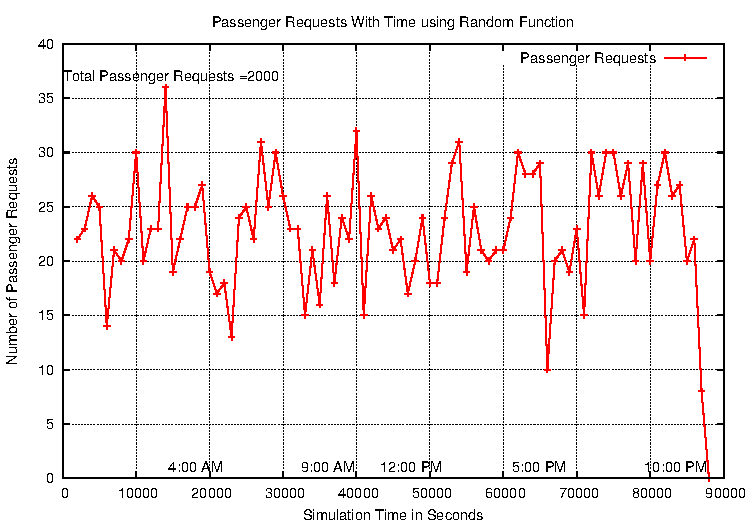
\includegraphics[scale=0.9]{../plots/passengerArrivalDistribution_old}
\caption{Passenger Arrival Requests modeled using random function}\label{fig:SVM}
\end{figure}

\begin{figure}[h!t]
\centering
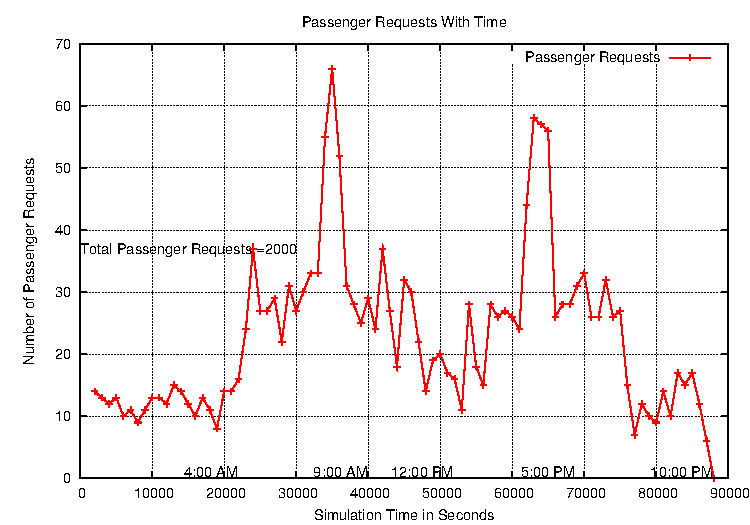
\includegraphics[scale=0.9]{../plots/passengerArrivalDistribution_9AM5PM}
\caption{Passenger Arrival Request modeled using customised function}\label{fig:SVM}
\end{figure}

\begin{figure}[h!t]
\centering
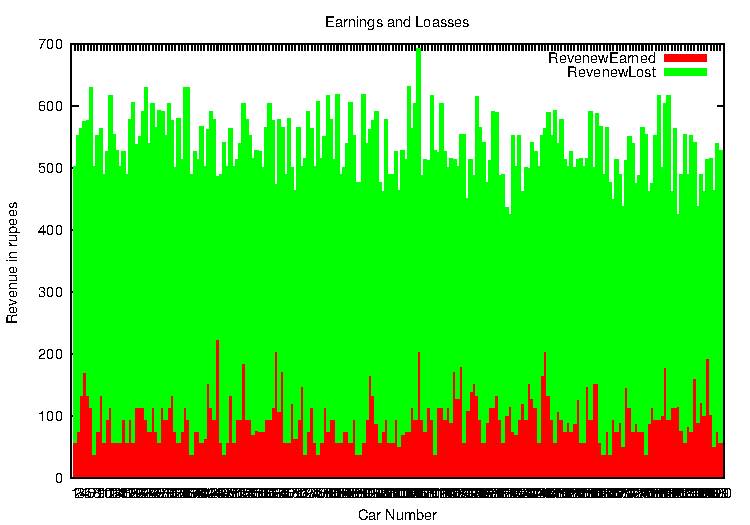
\includegraphics[scale=0.9]{../plots/EarnngsVsLosses}
\caption{Earnigs Vs Losses}\label{fig:SVM}
\end{figure}

\begin{figure}[h!t]
\centering
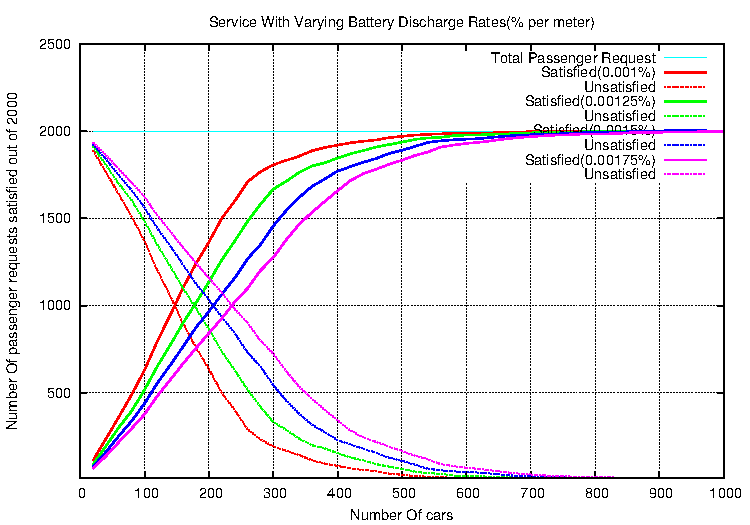
\includegraphics[scale=0.9]{../plots/nCarVariation_old}
\caption{Effect of Battery performance on service}\label{fig:SVM}
\end{figure}

\begin{figure}[h!t]
\centering
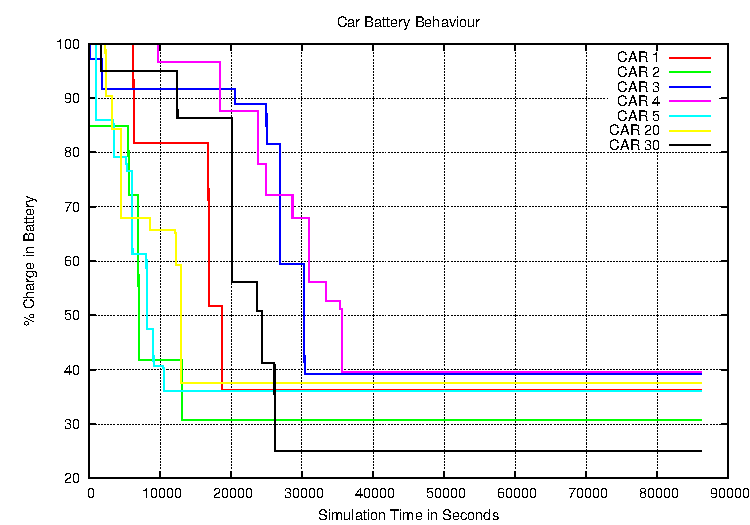
\includegraphics[scale=0.9]{../plots/carsBatteryPower}
\caption{Change in Battery charge with time}\label{fig:SVM}
\end{figure}
\indent sssssssssssssssssssssssssssssss


\chapter{Conclusion}
 sssssssssssssssssssssssssssssss
\subsection*{Acknowledgement}
I would like to thank Prof. Krithi Ramamrithm and Prof. Purushottam Kulkarni for their constant support and guidance.% to keep me motivated.

\appendix
\chapter{Forecasting accuracy gradient}

sssssssssssssssssssssssssssssss


\bibliographystyle{plainnat}
\bibliography{ref}
\end{document}
